\section{Research Plan} 
\label{sec:research}

% 30 pts for explanation here combined with timeline below

Having identified that we lack understanding of what information is redundant or necessary to meaningfully represent message passing with high volume Gantt charts, we must evaluate the visual notation we use to indicate message passing. To evaluate this notation we will perform a controlled experiment to evaluate how people perceive patterns and gauge the limitations of perception of those patterns. In order to generalize conclusions and mitigate the need for domain experts as subjects, this study will abstract away the literal use of a Gantt chart and represent patterns as lines connecting columns of rectangles.

\begin{figure}[h]
    \centering
    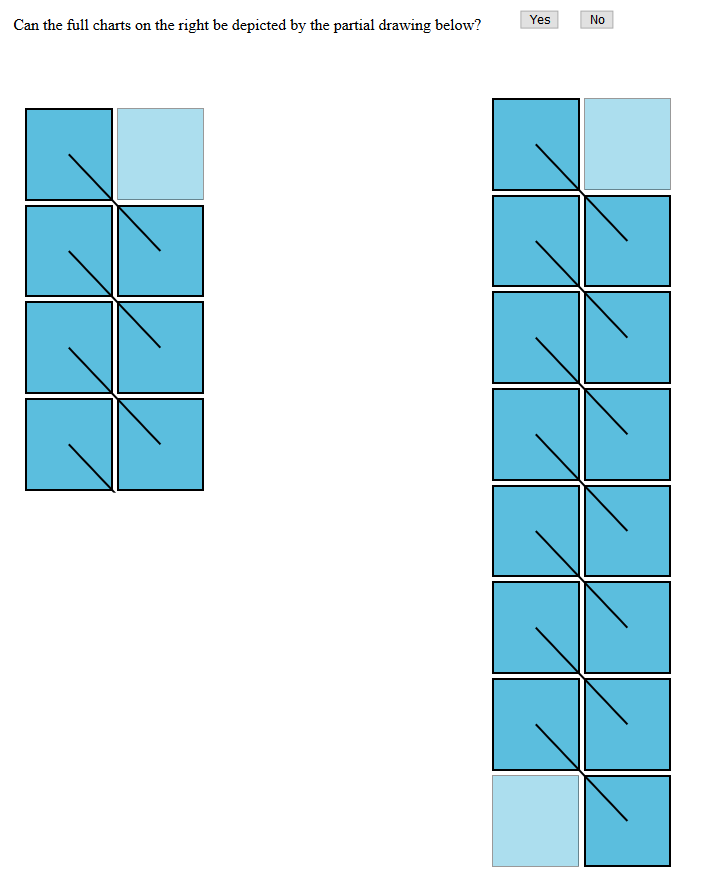
\includegraphics[width=.4\textwidth]{figs/study.png}
    \caption{The current design of the experiment software subjects will interact with. Users are presented with two images of connected columns and asked to compare the patterns of lines within each.}
    \label{fig:study}
\end{figure}


The intended experiment will be a within-subjects experiment with two independent variables comprised of two conditions and 4 conditions respectively. Users will be asked to compare a provided visualization of lines connecting boxes and compare it against another similar visualization. The first independent variable will be how much information we provide users to compare with: a partial rendering of the pattern or full rendering. Users will respond yes or no as to whether the provided pattern matches with a comparator we will swap out at random. The second independant variable will be the pattern itself, which could be one of four: a basic offset, a ring, a stencil, and an exchange. Examples of these patterns can be seen in Figure \ref{fig:patterns}. The dependant variable we measure from these responses is error rate -- how successfully users compared patterns in the face of. An example of the experiment layout can be seen in Figure \ref{fig:study}.


\begin{figure*}[t!]
     \subfloat[An example of an offset pattern.\label{fig:offset}]{%
       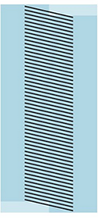
\includegraphics[width=0.2\textwidth, height=0.3\textwidth]{figs/offset_normal.png}
     }
     \hfill
     \subfloat[An example of an ring pattern. \label{fig:ring}]{%
       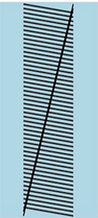
\includegraphics[width=0.2\textwidth, height=0.3\textwidth]{figs/ring_normal.png}
     }
    \hfill
    \subfloat[An example of a stencil pattern.\label{fig:stencil}]{%
       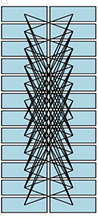
\includegraphics[width=0.2\textwidth, height=0.3\textwidth]{figs/trace_normalized.png}
     }
     \hfill
     \subfloat[An example of a exchange pattern.\label{fig:exchange}]{%
       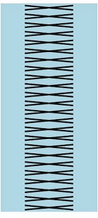
\includegraphics[width=0.2\textwidth, height=0.3\textwidth]{figs/exchange_normal.png}
     }
    \caption{Examples of various execution trace patterns.}
    \label{fig:patterns}
\end{figure*}

By measuring error rate, we will draw a connection between how much context a user is provided and if it is too much or too little to make meaningful conclusions. The experiment itself will be piloted with students from the University of Arizona who will also be asked to vocalize their inner thought processes so that we can better understand how the dependant variable is influenced by changes to the independent variable. From this pilot study we will to iterate on the design of this experiment to address weak points. From there, we will bring this study to the Supercomputing conference and collect data from the large population of attendees.

This large volume of collected data will be transformed and analyzed for validity using a statistical test. The derived error rates, being ratio data, will be analyzed with an ANOVA analysis to prove that experiment results are statistically significant. From here we will derive conclusions on what specific characteristics lead to higher or lower error rates by respondents, if possible.


% 5 pts
\subsection{Data}
\label{sec:data}

The data being used for this experiment is manufactured to produce the visualizations which subjects will be asked to compare. It is JSON encoded descriptions of the visual structure of question charts and corresponding comparison charts. This data is parsed and visualized by the experiment software. Some question/answer pairs have been provided by the project PI, however more will be produced as part of this experiment. 

% 15 pts
\subsection{Evaluation}
\label{sec:eval}
As alluded to above in Section \ref{sec:research}, this experiment will be evaluated with formal hypothesis testing. Hypothesis testing describes the process of performing statistical tests on experiment data to disprove the \textit{null hypothesis}. This hypothesis states that the independent variable(s) had no affect on the dependant variable(s) and that the results were completely random. By disproving this hypothesis we conclude that swapping out conditions in our independent variables did have some measurable effect on how subjects behaved. Anticipating that our error rates are ratio data, and expecting a normal distribution on that data, we plan to use an ANOVA analysis for this hypothesis testing. This plan could change as data is collected and a different test is deemed more appropriate. 

On a longer timescale, we expect to integrate the conclusions drawn from this study into a larger design study on Gantt charts. By building a visualization using ideas developed from this study we can validate those conclusions with the effectiveness of newly designed charts. And the effectiveness of these charts, can | in turn | be validated with various metrics such as community adoption rates, formal usability experiments, and comparative performance evaluations. The success of a new visualization or representation of communications in these charts would provide significant validation for the work proposed in this document.


% 5 pts
\subsection{Technology}
\label{sec:tech}

The core experiment platform which runs the experiment is a web application primarily coded in Javascript, HTML and CSS. D3js is used to execute the programmatic drawing of boxes and connecting lines. Data management functionality, like collection of user responses, saving and processing data is managed on the server side with python scripts. The \textit{flask} python library is used for serving down web pages and communicating with the client. These technologies are very commonly used in client server architectures and provide a robust means to quickly develop and iterate on an experiment platform which has a limited range of user interaction and minimal performance needs.

\subsection{Timeline}
\label{sec:timeline}

\vspace{1.5ex}\noindent\textbf{Project Milestone Two} 
For the second project milestone, experimental methodology will be expanded on and explained in greater detail. Any changes to the proposed independent and dependent variables will be noted with clear explanations of what provoked these changes and what better information can be gleaned from the experiment with these changes. Current development on the experiment platform should be complete enabling the execution of a pilot study on location at the University of Arizona. Full descriptions of the experiment platform and how it works will be included in the report at this milestone. Related works and background will be updated to reflect the author's research and expanded understanding of this domain.

\vspace{1.5ex}\noindent\textbf{Project Milestone Three}
By this project milestone, data will have been collected from the pilot study executed after milestone two. This data will be analyzed and presented alongside derived conclusions in this report. Planned changes to the experiment design resulting from this pilot experiment  will highlighted here. Changes to the experiment platform will also be detailed in this report and will be justified in the context of the pilot study. The experiment platform should be containerized at this juncture using Docker or some other technology and hosted on a server for general access. 

\vspace{1.5ex}\noindent\textbf{Project Milestone Four} 
By this milestone, the changes to the experiment design and experiment platform will be fully integrated into the project. A working and robust version of this software will be made available at the Supercomputing conference and a large scale experiment will be executed. Expectations and hypotheses will be outlined in the corresponding report and project progress will be detailed here.


\vspace{1.5ex}\noindent\textbf{Project Milestone Five} 
At this project milestone, data collected from a attendees to the Supercomputing conference will be aggregated, aligned, visualized and tested for statistical significance. Conclusions will be drawn from this data and reported on. Depending on the results of this experiment, the next steps will be clearly outlined in this report whether it is another iteration on this experiment's design or the application of derived conclusions.





\begin{table}[h]
%% Table captions on top in journal version
 \caption{Project Milestones}\vspace{1ex} % the \vspace adds some space after the top caption
 \label{tab:milestones}
 \scriptsize
 \centering % avoid the use of \begin{center}...\end{center} and use \centering instead (more compact)
   \begin{tabular}{l|p{.75\linewidth}}
     Milestone & Description (\%)\\
   \hline
     PM2 & Current development on the experiment platform complete, code available in online repository, experiment design more clearly articulated\\
     PM3 & Pilot study executed, data analyzed and conclusions drawn, proposals of adjustments to study design and software, software hosted on a server\\
     PM4 & Changes to study design and software fully implemented, initial data collected from large study, pre-experiment expectations and hypotheses clearly outlined\\
     PM5 & data analysis on data collected in milestone 4, conclusions drawn, clear plan on this study's iteration or adaptation of lessons learned\\
   \end{tabular}
\end{table}

